\documentclass[12pt,letterpaper,titlepage,twoside,openright]{report} 

\usepackage{fourier}
\usepackage{setspace}
\usepackage{natbib}
\usepackage[inner=1.25in,outer=1.25in,top=1.25in,bottom=1.25in]{geometry}
\doublespacing
\usepackage{amsmath}
\usepackage{amssymb}
\usepackage{graphicx}
\usepackage{dpfloat}
\renewcommand{\thefigure}{\arabic{figure}}



%%%%%%%% Declarations %%%%%%%%%%%%%%%
\DeclareMathOperator{\Tr}{tr}
\newcommand{\loss}[1]{\mathcal L\left(#1\right)}
\newcommand{\T}{{\sf T}}
\newcommand{\E}[2][]{\mathbb E_{#1}\left[ #2\right]}    % expected value
\DeclareMathOperator*{\argmin}{arg\,min}

\newcommand{\sq}[1]{\lq#1\rq}
\newcommand{\ie}{\emph{i.e.}\;}
\newcommand{\eg}{\emph{e.g.}\;}

\begin{document}

\begin{titlepage}
\begin{center}

\vspace*{2cm}
\textbf{\uppercase{\large Inference of neuronal functional connectivity from partial correlations of spiking activity}}

\vspace{1.5cm}
A Dissertation Submitted to the Faculty of

\medskip
The Graduate School 

Baylor College of Medicine

\vspace{1.5cm}
In Partial Fulfillment of the 

Requirements for the Degree

of 

Doctor of Philosophy

by 

\bigskip
{\large Dimitri Yatsenko}

\vfill
Houston, Texas

September 2014

\end{center}
\end{titlepage}


%%%%%%%%% SIGNATURE PAGE

\begin{center}
\textbf{\uppercase{\large Approved by the dissertation committee}}

\vspace{9pt}
Signed \underline{\hspace{3in}}

\vspace{-9pt}
Andreas S.\ Tolias, Ph.D.

\vspace{-9pt}
Chairperson


Signed \underline{\hspace{3in}}

\vspace{-9pt}
Fabrizio Gabbiani, Ph.D.


Signed \underline{\hspace{3in}}

\vspace{-9pt}
Kre\v{s}imir Josi\`{c}, Ph.D.

Signed \underline{\hspace{3in}}

\vspace{-9pt}
Daoyun Ji, Ph.D.

Signed \underline{\hspace{3in}}

\vspace{-9pt}
Athanassios G.\ Siapas, Ph.D.


\vspace{24pt}
\textbf{\uppercase{\large Approved by the department of neuroscience}}

\vspace{9pt}
Signed \underline{\hspace{3in}}

\vspace{-9pt}
Paul J.\ Pfaffinger, Ph.D.

\vspace{-9pt}
Director of Graduate Studies

Signed \underline{\hspace{3in}}

\vspace{-9pt}
Dora E.\ Angelaki, Ph.D.

\vspace{-9pt}
Chairman of Department

\vspace{24pt}
\textbf{\uppercase{\large Approved by the dean of graduate sciences}}

\vspace{9pt}
Signed \underline{\hspace{3in}}

\vspace{-9pt}
Hiram F.\ Gilbert, Ph.D.

\vspace{6pt}
Date \underline{\hspace{3in}}

\end{center}

\chapter*{Acknowledgments}
\addcontentsline{toc}{chapter}{\numberline{}Acknowledgments}
My six years of graduate studies at Baylor College of Medicine have been a great privilege, challenge, and adventure. During this time, I received tremendous support from my mentors, instructors, sponsors, collaborators, labmates, administrative staff, and friends.

I am profoundly grateful to my supervisor, Dr.\ Andreas S.\ Tolias for allowing me to become part of the multidisciplinary research environment that he has built in his lab. From our first interview and throughout the many projects we have undertaken since, he has encouraged me to think boldly yet critically.  His optimism and enthusiasm made it possible to work through several uncertain phases of my projects and to define new goals.  I thank him for the freedom to explore and pursue my own ideas.

I thank the past and current members of my dissertation committee Drs.\ Fabrizio Gabbiani, Daoyun Ji, Peter Saggau, Kre\v{s}imir Josi\`c, and Athanassios G.\ Siapas  for their continued advice and guidance. In particular, Dr.\ Josi\`c became closely involved in the definition and verification of the major mathematical aspects of this dissertation.

This work was performed in close collaboration with my lab mates. In particular, Emmanouil Froudarakis sharing his two-photon imaging data to be included in this dissertation. Cathryn R.\ Cadwell provided transgenic mice with fluorescently labeled interneurons that were used in this study. I also thank my former labmate Dr.\ R.\ James Cotton who, in collaboration with Prof.~Peter Saggau, developed the unique two-photon microscope for high-speed \emph{in vivo} calcium imaging that enabled the level of analysis developed in this dissertation. I thank Alexander S.\ Ecker for critically examining the assumptions underlying my statistical models and helping eliminate several logical flaws early in the process.

The early stages of this  work were supported in part by a Predoctoral Fellowship from the Theoretical and Computational Neuroscience Training Program of the Gulf Coast Consortia.  The financial support and the excellent coursework and networking opportunities organized through this fellowship were instrumental in bringing this work to fruition. I am grateful to Dr.\ Valery Kalatsky at the University of Houston who served as my co-mentor during fellowship.

I also wish to express my gratitude to the BCM Neuroscience Department for running an excellent training program with great resources and opportunities available to its students.


\chapter*{Abstract}
\addcontentsline{toc}{chapter}{\numberline{}Abstract}
Current standard models of the brain's sensory circuits are derived from and supported by detailed empirical characterizations of the responses of individual neurons to external stimuli.
Single-unit statistical descriptions of neurons' stimulus response properties such as, for example, the \emph{receptive field} and \emph{feature selectivity} have proven immensely successful in defining the \emph{functional architecture} of neural circuits and systems: the relationship between response properties of individual cells and the anatomical organization of the circuits  \citep{Ohki:2005,Reid:2012}.
Yet neuroscientists have long recognized that the more intriguing brain functions must be expressed in the dynamic, recurrent interactions between neurons and in the emergent, intrinscially generated population activity that is not reducible to stimulus-driven response \citep{Yuste:2005}.
This recognition motivates ambitious technological developments to record the simultanous spiking activity of large populations of neurons in intact neural circuits \emph{Alivisatos:2013}. 
It is often taken for granted that large-scale recordings of the spiking activity of cells large-scale recordings of the spiking activity of cells 


\tableofcontents

\listoffigures

%\listoftables

\chapter{Introduction}
\clearpage 
\section{Single-cell descriptions of neural function}
A fortuitous fact of neurobiology is that the spiking activity of individual cells can we efficiently described as a function of external stimuli with simple statistical models with only a handful of parameters fitted to the data \citep{Carandini:2005}. From the original discovery and with subsequent refinement of such descriptions over the past 50+ years, constructs such as \emph{receptive fields} and \emph{orientation tuning} have become principal tools for defining the \emph{functional architecture} of sensory cortex, \emph{i.e.}\ the relationship between single-cell properties of neural function and the cell types, cortical layers, synaptic connectivity, and the physical arrangements of cells  \citep{Hubel:1962,Ohki:2005,Reid:2012}.

\section{Functional connectivity in multineuronal recordings}
Despite the remarkable success of single-cell descriptions of neural functions, neuroscientists have long recognized that the truly intriguing properties of brain function emerge in the interactions of cells between each other and the resulting intrinsically generated activity \citep{Yuste:2005}.  A major obstacle to investigating functional interactions in populations on neurons, 

\section{Functional connectivity in population calcium signals}


\chapter{Functional connectivity in neural circuits inferred from partial correlations}
This work has been submitted for publication as \citep{Yatsenko:2014}
\clearpage

Ambitious projects aim to record the activity of ever larger and denser neuronal populations \emph{in vivo}.  Correlations in neural activity measured in such recordings can reveal important aspects of  neural circuit organization.  However, estimating and interpreting large correlation matrices is statistically challenging.  Estimation can be improved by regularization, \emph{i.e.}\;by imposing a structure on the estimate.  The amount of improvement depends on how closely the assumed structure represents dependencies in the data. Therefore, the selection of the most efficient correlation matrix estimator for a given neural circuit must be determined empirically.  Importantly, the identity and structure of the most efficient estimator informs about the types of dominant dependencies governing the system.
We sought statistically efficient estimators of neural correlation matrices in recordings from large, dense groups of cortical neurons.  Using fast 3D random-access laser scanning microscopy of calcium signals, we recorded the activity of nearly every neuron in volumes 200 $\mu$m wide and 100 $\mu$m deep (150--350 cells) in mouse visual cortex.  We hypothesized that in these densely sampled recordings, the correlation matrix should be best modeled as the combination of a sparse graph of pairwise partial correlations representing interactions between the observed neuronal pairs and a low-rank component representing common fluctuations and external inputs.  Indeed, in cross-validation tests, the covariance matrix estimator with this structure consistently outperformed other regularized estimators. The sparse component of the estimate defined a graph of interactions. These interactions reflected the physical distances and orientation tuning properties of cells: The density of positive `excitatory' interactions decreased rapidly with geometric distances and with differences in orientation preference whereas negative `inhibitory' interactions were less selective.  Because of its superior performance, this `sparse + latent' estimator likely provides a more physiologically relevant representation of the functional connectivity in densely sampled recordings than the sample correlation matrix.

\section{Introduction}
\emph{Functional connectivity} is a statistical description of observed \emph{multineuronal} activity patterns not reducible to the response properties of the individual cells. Functional connectivity reflects local synaptic connections, shared inputs from other regions, and endogenous network activity. Although functional connectivity is a phenomenological description without a strict mechanistic interpretation, it can be used to generate hypotheses about the anatomical architecture of the neural circuit and to test hypotheses about the processing of information at the population level.

Pearson correlations between the spiking activity of pairs of neurons are among the most familiar measures of functional connectivity \citep{Averbeck:2006, Zohary:1994, Kohn:2005, Bair:2001, Ecker:2010}.  In particular, \emph{noise correlations}, \emph{i.e.}\;the correlations of trial-to-trial response variability between pairs of neurons, have a profound impact on stimulus coding \citep{Zohary:1994, Abbott:1999, Sompolinsky:2001, Nirenberg:2003, Averbeck:2006, Josic:2009, Berens:2011, Ecker:2011}. In addition, noise correlations and correlations in spontaneous activity have been hypothesized to reflect aspects of synaptic connectivity \citep{Gerstein:1964}.  Interest in neural correlations has been sustained by a series of discoveries of their nontrivial relationships to various aspects of circuit organization such as the physical distances between the neurons \citep{Smith:2008, Denman:2013}, their synaptic connectivity \citep{Ko:2011},  stimulus response similarity \citep{Bair:2001, Arieli:1995, Chiu:2002, Kenet:2003, Kohn:2005, Cohen:2008, Cohen:2009, Ecker:2010, Rothschild:2010, Ko:2011, Smith:2013b}, cell types \citep{Hofer:2011}, cortical layer specificity \citep{Hansen:2012, Smith:2013}, progressive changes in development and in learning \citep{Golshani:2009, Gu:2011, Ko:2013}, changes due to sensory stimulation and global brain states \citep{Greenberg:2008, Goard:2009, Kohn:2009, Rothschild:2010, Ecker:2014, Renart:2010}.

Neural correlations do not come with ready or unambiguous mechanistic interpretations. They can arise from monosynaptic or polysynaptic interactions, common or correlated inputs, oscillations, top-down modulation, and background network fluctuations, and other mechanisms \citep{Perkel:1967, Moore:1970, Shadlen:1998, Salinas:2001, Ostojic:2009, Rosenbaum:2011}. But multineuronal recordings do provide more information than an equivalent number of separately recorded pairs of cells. For example, the eigenvalue decomposition of the covariance matrix expresses shared correlated activity components across the population; common fluctuations of population activity may be accurately represented by only a few eigenvectors that affect all correlation coefficients. On the other hand, a correlation matrix can be specified using the \emph{partial correlations} between pairs of the recorded neurons. The partial correlation coefficient between two neurons reflects their linear association conditioned on the activity of all the other recorded cells \citep{Whittaker:1990}.  Under some assumptions, partial correlations measure conditional independence between variables and may more directly approximate causal effects between components of complex systems than correlations \citep{Whittaker:1990}. For this reason, partial correlations have been used to describe interactions between genes in functional genomics \citep{Schafer:2005, Peng:2009} and between brain regions in imaging studies \citep{Varoquaux:2012, Ryali:2012}. These opportunities have not yet been explored in neurophysiological studies where most analyses have only considered the distributions of pairwise correlations \citep{Zohary:1994, Bair:2001, Smith:2008, Ecker:2010}.

However, estimation of correlation matrices from large populations presents a number of numerical challenges. The amount of recorded data grows only linearly with population size whereas the number of estimated coefficients increases quadratically. This mismatch leads to an increase in spurious correlations, overestimation of common activity (\emph{i.e.}\;overestimation of the largest eigenvalues) \citep{Ledoit:2004}, and poorly conditioned partial correlations \citep{Schafer:2005}. The \emph{sample correlation matrix} is an unbiased estimate of the true correlations but its many free parameters make it sensitive to sampling noise. As a result, on average, the sample correlation matrix is farther from the true correlation matrix than some structured estimates.

Estimation can be improved through \emph{regularization},  the technique of deliberately imposing a structure on an estimate in order to reduce its estimation error \citep{Schafer:2005, Bickel:2006}. To `impose a structure' on an estimate means to bias (`shrink') it toward a reduced representation  with fewer free parameters, the \emph{target estimate}.   The optimal target estimate and the optimal amount of shrinkage can be obtained from the data sample either analytically \citep{Ledoit:2003, Ledoit:2004, Schafer:2005}  or by cross-validation \citep{Friedman:1989}. An estimator that produces estimates that are, on average, closer to the truth for a given sample size is said to be more \emph{efficient} than other estimators.

Although regularized covariance matrix estimation is commonplace in finance \citep{Ledoit:2003}, functional genomics \citep{Schafer:2005}, and brain imaging \citep{Ryali:2012}, surprisingly little work has been done to identify optimal regularization of neural correlation matrices.

Improved estimation of the correlation matrix is beneficial in itself. For example, improved estimates can be used to optimize  decoding of the population activity \citep{Friedman:1989, Berens:2012}. But reduced estimation error is not the only benefit of regularization.  Finding the most efficient among many regularized estimators leads to insights about the system itself: the structure of the most efficient estimator is a parsimonious representation of the regularities in the data.

The advantages due to regularization increase with the size of the recorded population. With the advent of  big neural data \citep{Alivisatos:2013}, the search for optimal regularization schemes will become increasingly relevant in any model of population activity. Since optimal regularization schemes are specific to systems under investigation, the inference of functional connectivity in large-scale neural data will entail the search for optimal regularization schemes. Such schemes may involve combinations of heuristic rules and numerical techniques specially designed for given types of neural circuits.

What structures of correlation matrices best describe the multineuronal activity in specific circuits and in specific brain states?  More specifically, are correlations in the visual cortex during visual stimulation best explained by common fluctuations or by local interactions within the recorded microcircuit?

To address these questions, we evaluated four regularized covariance matrix estimators that imposed different structures on the estimate. The estimators are designated as follows:
\begin{description}
\item[$C_{\sf sample}$] -- sample covariance matrix, the unbiased, unregularized estimator.
\item[$C_{\sf diag}$] -- linear shrinkage of covariances toward zero, \emph{i.e.}\;toward a diagonal covariance matrix.
\item[$C_{\sf factor}$] -- a low-rank approximation of the sample covariance matrix, representing inputs from unobserved shared factors (latent units).
\item[$C_{\sf sparse}$] -- sparse partial correlations, \emph{i.e.}\;a large fraction of the \emph{partial} correlations between pairs of neurons are set to zero.
\item[$C_{\sf sparse+latent}$] -- sparse partial correlations between the recorded neurons \emph{and} linear interactions with a number of latent units.
\end{description}

First, we used simulated data to demonstrate that the selection of the optimal estimator indeed pointed to the true structure of the dependencies in the data.

We then performed a cross-validated evaluation to establish which of the four regularized estimators was most efficient for representing the population activity of dense groups of neurons in mouse primary visual cortex recorded with high-speed 3D random-access two-photon imaging of calcium signals. In our data, the sample correlation coefficients were largely positive and low.  We found that the best estimate of the correlation matrix was $C_{\sf sparse+latent}$.  This estimator revealed a sparse network of partial correlations (`{interactions'), between the observed neurons; it also inferred latent units exerting linear effects on the observed neurons. We analyzed these networks of partial correlations and found the following: Whereas significant noise correlations were predominantly positive, the inferred interactions had a large fraction of negative values possibly reflecting inhibitory circuitry.  Moreover, we found that these interactions exhibited a stronger relationship to the physical distances and to the differences in preferred orientations than noise correlations. In contrast, the inferred negative interactions were less selective.

\section*{Results}
\subsection*{Covariance estimation}
The covariance matrix is defined as
\begin{equation}\label{eq:true-covariance}
    \Sigma = \E{(x-\mu)(x-\mu)^\T},\quad \mu = \E{x}
    \end{equation}
    where $\E{\cdot}$ denotes expectation; the $p\times 1$ vector $x$ is a single observation of the firing rates of $p$ neurons in a time bin of some duration; and $\mu$ is the vector of expected firing rates. 

Given a set of observations $\{x(t): t\in T$\} of population activity, where $x(t)$ is a $p\times 1$ vector of firing rates in time bin $t$, and an unbiased estimate $\bar x$ of the mean activity, the \emph{sample covariance matrix} is
\begin{equation}\label{eq:sample}
    C_{\sf sample} = \frac 1 n \sum\limits_{t\in T} (x(t)-\bar x)(x(t)-\bar x)^\T,
    \end{equation}
where $n$ is the number of time bins in $T$. 
The sample covariance matrix is an unbiased estimate of the covariance matrix ($\E{C_{\sf sample}}=\Sigma$) provided that the estimate of the mean, $\bar x$, is known or is already estimated from an independent dataset. 
When the mean is estimated from the same sample, $C_{\sf sample}$ becomes biased toward zero.  However, in all the cases where unbiasedness is required, we will estimate the mean from a separate sample.

Given any covariance matrix estimate $C$, the corresponding correlation matrix $R$ is calculated by normalizing the rows and columns of $C$ by the square roots of its diagonal elements to produce unit entries on the diagonal:
\begin{equation}\label{eq:precision}
    R = (\mbox{diag}(C))^{-\frac 1 2} C (\mbox{diag}(C))^{-\frac 1 2},
\end{equation}
where $\mbox{diag}(C)$ denotes the diagonal matrix with the diagonal elements from $C$.

The \emph{partial correlation} between a pair of variables is the Pearson correlation coefficient of the residuals of the linear least-squares predictor of their activity based on all the other variables, excluding the pair \citep{Anderson:2003, Whittaker:1990}. Partial correlations figure prominently in probabilistic \emph{graphical modeling} wherein the joint distribution is explained by sets of two-way interactions \citep{Whittaker:1990}. For the multivariate Gaussian distribution, zero partial correlations indicate conditional independence of the pair, implying a lack of direct interaction \citep{Dempster:1972, Whittaker:1990}. More generally, partial correlations can serve as a measure of conditional independence under the assumption that most dependencies in the system include strong linear effects \citep{Whittaker:1990,Baba:2004}. As neural recordings become increasingly dense, partial correlations may prove useful as indicators of conditional independence (lack of functional connectivity) between pairs of neurons.

Pairwise partial correlations are closely related to the elements of the \emph{precision matrix}, \emph{i.e.}\;the inverse of the covariance matrix \citep{Dempster:1972,Whittaker:1990}. Zero elements in the precision matrix signify zero partial correlation between the two variables. Given the covariance estimate $C$, the matrix of partial correlations $P$ is computed by normalizing the rows and columns of the \emph{precision matrix} $C^{-1}$ to produce negative unit entries on the diagonal:
\begin{equation}\label{eq:partial}
    P = -\left(\mbox{diag}(C^{-1})\right)^{-\frac 1 2} C^{-1} \left(\mbox{diag}(C^{-1})\right)^{-\frac 1 2}
\end{equation}

Increasing the number of recorded neurons results in a higher \emph{condition number} of the covariance matrix \cite{Ledoit:2004} making the partial correlation estimates \emph{ill-conditioned}: small errors in the covariance estimates translate into much greater errors in the estimates of partial correlations. With massively multineuronal recordings, partial correlations cannot be estimated without \emph{regularization} \cite{Ledoit:2004,Schafer:2005}.

We considered four regularized estimators based on distinct families of target estimates: $C_{\sf diag}$, $C_{\sf factor}$, $C_{\sf sparse}$, and $C_{\sf sparse+latent}$. In probabilistic models with exclusively linear dependencies, the target estimates of these estimators correspond to distinct families of graphical models (Fig.~\ref{fig:1} Row 1).

\begin{figure}
\begin{leftfullpage}
\caption[Regularized correlation matrix estimators]{{\bf Regularized correlations matrix estimators.}
{\bf Regularized estimators whose structure matches the true structure in the data are more efficient.}
     {\bf Row 1.} Graphical models of the target estimates of the four respective regularized covariance matrix estimators.  Recorded neurons are represented by the green spheres and latent units by the lightly shaded spheres.  Edges represent conditional dependencies, \emph{i.e.}\;`interactions'.
     {\bf Row 1, A}.  For estimator $C_{\sf diag}$, the target estimate is a diagonal matrix, which describes systems that lack linear dependencies.
     {\bf  Row 1, B.} For estimator $C_{\sf factor}$, the target estimate is a factor model (low-rank matrix plus a diagonal matrix), representing systems in which correlations arise due to common input from latent units.
     {\bf  Row 1, C}. For estimator $C_{\sf sparse}$, the covariance matrix is approximated as the inverse of a sparse matrix. This approximation describes systems in which correlations arise from a sparse set of  linear associations between the observed units.
     {\bf  Row 1, D}.  For estimator $C_{\sf sparse+latent}$, the covariance matrix is approximated as the inverse of the sum of a sparse matrix and a low-rank matrix. This approximation describes a model wherein correlations arise due to sparse associations between the recorded cells \emph{and} due to several latent units.
     \\
     {\bf Row 2:} Examples of $50\times 50$ correlation matrices corresponding to each structure: {\bf A.} the diagonal correlation matrix, {\bf B.} a factor model with four latent units, {\bf C.}  a correlation matrix with 67\%  off-diagonal zeros in its inverse, and {\bf  D.} a correlation matrix whose inverse is the sum of a rank-3 matrix (\emph{i.e.}\;three latent units) and a sparse matrix with 76\% off-diagonal zeros.
     \\
{\bf Row 3:} Sample correlation matrices calculated from samples of size $n=500$ drawn from simulated random processes with respective correlation matrices shown in Row 2.  The structure of the sample correlation matrix is difficult to discern by eye.
     \\
{\bf Row 4:} Estimates computed from the same data as in Row 3 using structured estimators of the matching type: $C_{\sf diag}$ when the ground truth was diagonal in column A, $C_{\sf factor}$ when the ground truth is a factor model in column B, $C_{\sf sparse}$ when the ground truth has a sparse precision matrix in column C, and $C_{\sf sparse+latent}$ when the ground truth has both latent units and sparse linear interactions between observed units in column C.  Regularization was optimized by cross-validation. 
The regularized estimates are closer to the truth than the sample correlation matrices.
     \\
{\bf Row 5:} True loss (Eq.~\ref{eq:loss}) for the five estimators as a function of sample size. The error bars indicate the standard deviation of the mean.  Estimators with structure that matches the true model converged to zero faster than the other estimators.
     \\
{\bf Row 6:} Validation loss (Eq.~\ref{eq:vloss}) for the five estimators relative to the matching estimators for each type of ground truth. Error bars indicate the standard deviation of the mean.  Differences in validation loss approximate differences in true loss.
}\label{fig:1}
\end{leftfullpage}
\end{figure}

\begin{figure}
\begin{fullpage}
        \includegraphics[width=\textwidth]{./figures/Figure1.png}
\end{fullpage}
\end{figure}
  %%%%%% FIGURE 1 from the paper

The target estimate of estimator $C_{\sf diag}$ is the diagonal matrix $D$ containing estimates of neurons' variances. Regularization is achieved by linear \emph{shrinkage} of the sample covariance matrix toward $D$, controlled by the scalar \emph{shrinkage intensity} parameter $\lambda \in [0, 1]$:
\begin{equation}\label{eq:c-diag}
C_{\sf diag} = (1-\lambda) C_{\sf sample} + \lambda D
\end{equation}
The structure imposed by $C_{\sf diag}$ favors (performs better with) populations with no linear associations between the neurons (Fig.~\ref{fig:1} Row 1, A).  If sample correlations are largely spurious, $C_{\sf diag}$ is expected to be more efficient than other estimators.

Estimator $C_{\sf factor}$ approximates the covariance matrix by the factor model,
\begin{equation}\label{eq:c-factor}
C_{\sf factor} = L + D,
\end{equation}
where $L$ is a $p\times p$ symmetric positive semidefinite matrix with low rank and $D$ is a diagonal matrix.
This approximation is at the basis of \emph{factor analysis} \citep{Anderson:2003}. 
In factor analysis, matrix $L$ represets covariances arising from latent factors with the rank of $L$ indicating the number of such latent variables.
Matrix $D$ contains the variances of the independent noise in the observed variables.
The estimator is regularized by the selection of the rank of $L$. 
The structure imposed by $C_{\sf factor}$ favors conditions in which the population activity is linearly driven by a number of latent factors that affect many cells while direct interactions between the recorded cells are insignificant (Fig.~\ref{fig:1} Row 1, B).

Estimator $C_{\sf sparse}$ is produced by approximating the precision matrix by a sparse matrix $S$:
\begin{equation}\label{eq:c-sparse}
C_{\sf sparse} = S^{-1}.
\end{equation}
where $S$ is a sparse matrix, \ie many of its off-diagonal elements are forced to zero. The estimator is regularized by adjusting the sparsity (fraction of off-diagonal zeros) in $S$. 
Zeros in the precision matrix coincide with zero partial correlations between the same pairs of variables.  
Under the assumption of linearity of interactions in the system, zero partial correlation indicates conditional independence or lack of direct interaction between the pair of variables.
Therefore, the structure imposed by $C_{\sf sparse}$ favors conditions in which neural correlations arise from direct linear effects (`interactions') between some pairs of the observed neurons (Fig.~\ref{fig:1}} Row 1, C).
The problem of finding the optimal set of non-zero elements of the precision matrix is known as \emph{covariance selection} \citep{Dempster:1972}. 

Estimator $C_{\sf sparse+latent}$ is obtained by approximating the precision matrix as the sum of a sparse component and a low-rank component:
\begin{equation}\label{eq:c-sl}
C_{\sf sparse+latent} = (S - L)^{-1},
\end{equation}
where $S$ is a sparse matrix and $L$ is a low-rank symmetric positive semidefinite matrix. 
The estimator is regularized by adjusting the sparsity of $S$ (sparsity of local interactions) and the rank of $L$ (number of latent units) 
See Methods for a more detailed explanation. 
The structure imposed by $C_{\sf sparse+latent}$ favors conditions in which the activity of neurons is determined by linear effects between some observed pairs of neurons and some from several latent units (Fig.~\ref{fig:1} Row 1, D) \citep{Chandrasekaran:2010,Ma:2013}.

\subsection{Simulation}
We next demonstrate how the most efficient among different regularized estimators can reveal the structure of correlations.
We constructed four families of $50\times 50$ covariance matrices, each with structure that matched one of the four regularized estimators (Fig.~\ref{fig:1} Row 2, A--D and Methods).  We used these covariance matrices as the ground truth in multivariate Gaussian distributions with zero means and drew samples of various sizes. 
The sample correlation matrices from finite samples (\emph{e.g.}\ $n=500$ in Fig.~\ref{fig:1} Row 3) were contaminated with sampling noise and their underlying structures were difficult to discern.

The evaluation of any covariance matrix estimator, $C$, is performed with respect to a \emph{loss function} $\ell(C,\Sigma)$ to quantify its discrepancy from the truth, $\Sigma$.  The loss function is chosen to attain its minimum when $C=\Sigma$.
Here, in the role of the loss function we adopted the Kullback-Leibler divergence between multivariate normal distributions with equal means, scaled by $\frac 1 p$ to make its values comparable across different population sizes: 
\begin{equation}\label{eq:loss}
    \ell(C,\Sigma) = 
    \frac 1 p D_{KL}\left(\mathcal N_\Sigma\,\Vert\,\mathcal N_C\right) = 
    \frac 1 {2p} \left[\Tr(C^{-1}\Sigma) + \ln\det C - \ln\det\Sigma - p\right] 
\end{equation}
Therefore, $\ell(C,\Sigma)$ is expressed in nats/neuron per time bin.

We drew 30 independent samples with sample sizes $n=250$, 500, 1000, 2000, and 4000 from each model and computed the loss $\ell(C,\Sigma)$ for each of the five estimators.  
The hyperparameters of the regularized estimators were optimized by nested cross-validation using only the data in the sample.  
All the regularized estimators produced better estimates (lower loss) than the sample covariance matrix.  
However, estimators whose structure matched the true model outperformed the other estimators (Fig.~\ref{fig:1} Row 5).

Note that when the ground truth had zero correlations (Column A), $C_{\sf factor}$ performed equally well to $C_{\sf diag}$ because it correctly inferred zero factors and only estimated the individual variances. 
Similarly, when the number of latent units was zero (Column C), $C_{\sf sparse+latent}$ performed nearly equally well to $C_{\sf sparse}$ because it correctly inferred zero latent units.
With increasing sample sizes, all estimators converged to the ground truth (zero loss) but the estimators with correct structure outperformed the others even for large samples.

In more realistic conditions, when the ground truth is not accessible, the loss cannot be computed directly but may be estimated from data through \emph{validation}.
In a validation procedure, a validation sample covariance matrix $C_{\sf sample}^\prime$ is computed from a testing data set that is independent from the data used for computing $C$.
Then the \emph{validation loss} $\loss{C,C^\prime_{\sf sample}}$ measures the discrepancy of $C$ from $C^\prime_{\sf sample}$. 
Here, in the role of validation loss, we adopted the negative multivariate normal log likelihood of $C$ given $C^\prime_{\sf sample}$, also scaled by $\frac 1 p$ and omitting the constant term: 
\begin{equation}\label{eq:vloss}
    \loss{C,C^\prime_{\sf sample}} = \frac 1 {2p} \left[\Tr(C^{-1}C^\prime_{\sf sample})+\ln\det C \right]
\end{equation}

Since $\loss{\cdot,\cdot}$ is additive in its second argument and $C^\prime_{\sf sample}$ is an unbiased estimate of $\Sigma$, then, for given $C$ and $\Sigma$, the validation loss is an unbiased estimate of the true loss, up to a constant:
\begin{equation}
    \E{\loss{C,C_{\sf sample}^\prime}}=\loss{C,\E{C_{\sf sample}^\prime}}=\loss{C,\Sigma} = \ell(C,\Sigma) + \mbox{const}.
\end{equation}
Therefore, the validation procedure allows comparing the relative values of loss of different covariance estimators.

Indeed, the validation loss computed by 10-fold cross-validation (see Methods) accurately reproduced the relative values of the true loss and the rankings of the covariance estimators without access to the ground truth (Fig.~\ref{fig:1} Row 6). 

In the example above, the data were sampled from  multivariate normal random variables. In such models, partial correlations perfectly characterize the conditional dependencies between variables and the graphical models of partial correlations exactly correspond to the conditional dependencies in the data. 
To demonstrate that estimator rankings were robust to deviations from Gaussian models, we repeated the same cross-validated evaluation using pairwise Ising models to generate the data.

Ising models have been used to infer functional connectivity from neuronal spike trains \citep{Hertz:2011}. 
Conveniently, the Ising model has equivalent mathematical form to the Gaussian distribution,
\begin{equation}\label{eq:ising}
    x\sim \frac 1 {Z(J,h)} \exp\left(\frac 1 2 x^\T J x + h^\T x \right)
\end{equation}
but the Ising model is defined on the multivariate binary domain rather than the continuous domain. 
Both models are maximum-entropy models constrained to match the mean firing rates and the covariance matrix \citep{Jaynes:1957}.
The partition function $Z(J,h)$ normalizes the distribution on the models' respective domains. 
In the Gaussian model, the matrix $-J^{-1}$ is the covariance matrix; and the mean values are $\mu=J^{-1}h$.  
For the Ising model, $J$ is the matrix of pairwise interactions and $h$ is the vector of the cells' individual activity drives, although they do not have a simple relationship to the means and the covariance matrix. 
Both distributions have the same structure of pairwise conditional dependencies: zeros in the matrix $J$ indicate conditional independence between the corresponding pair of neurons. 

\begin{figure}
\begin{leftfullpage}
\caption[Estimation of noise correlations from population calcium signals]
{{\bf Estimation of noise correlations from population calcium signals.}
Visual stimuli comprising full-field drifting gratings interleaved with blank screens ({\bf A}) presented during two-photon recordings of somatic calcium signals using fast 3D random-access microscopy ({\bf B}).
{\bf C--F.} Calcium activity data from an example site.
{\bf C.} Representative calcium signals of seven cells, downsampled to 20 Hz, out of the 292 total recorded cells. Spiking activity inferred by nonnegative deconvolution is shown by red ticks below the trace.
{\bf D.} The spatial arrangement and orientation tuning of the 292 cells from the imaged site. The cells' colors indicate their orientation preferences. The gray cells were not significantly tuned.
{\bf E.} The sample noise correlation matrix of the activity of the neural population.
{\bf F.} Histogram of noise correlation coefficients in one site. The red line indicates the mean correlation coefficient of 0.020.
} \label{fig:2}
\end{leftfullpage}
\end{figure}

\begin{figure}
\begin{fullpage}
        \begin{center}
        \includegraphics[height=\textheight]{./figures/Acquisition.pdf}
        \end{center}
\end{fullpage}
\end{figure}
  %%%%%% FIGURE 2 from the paper

Indeed, despite their considerable departure from strictly linear conditional dependencies, Ising models yielded the same relationships between the performances of the covariance estimators as the Gaussian models in cross-validation (Fig.~\ref{fig:2}). Identical interaction matrices $J$  of the joint distributions over the observable and latent variables were used for both the Gaussian and the Ising models.

This simulation study demonstrated that cross-validated evaluation of regularized estimators of the covariance matrix of population activity can discriminate between structures of dependencies in the population. The identity of the most efficient covariance estimator for a particular neural circuit is therefore an empirical finding characterizing the nature of circuit  interactions.

\subsection{The $C_{\sf sparse+latent}$ estimator is most efficient in neural data}
\begin{figure}
\begin{leftfullpage}
\caption[Estimation of noise correlations from population calcium signals]
{{\bf Estimation of noise correlations from population calcium signals.}
Visual stimuli comprising full-field drifting gratings interleaved with blank screens ({\bf A}) presented during two-photon recordings of somatic calcium signals using fast 3D random-access microscopy ({\bf B}).
{\bf C--F.} Calcium activity data from an example site.
{\bf C.} Representative calcium signals of seven cells, downsampled to 20 Hz, out of the 292 total recorded cells. Spiking activity inferred by nonnegative deconvolution is shown by red ticks below the trace.
{\bf D.} The spatial arrangement and orientation tuning of the 292 cells from the imaged site. The cells' colors indicate their orientation preferences. The gray cells were not significantly tuned.
{\bf E.} The sample noise correlation matrix of the activity of the neural population.
{\bf F.} Histogram of noise correlation coefficients in one site. The red line indicates the mean correlation coefficient of 0.020.
} \label{fig:2}
\end{leftfullpage}
\end{figure}

\begin{figure}
\begin{fullpage}
        \begin{center}
        \includegraphics[height=\textheight]{./figures/Acquisition.pdf}
        \end{center}
\end{fullpage}
\end{figure}
    %%%%% FIGURE 2 from the paper 
We recorded the calcium activity of densely sampled populations of neurons in the supragranular layers in primary visual cortex of fentanyl-anesthetized mice using fast random-access 3D scanning two-photon microscopy during visual stimulation (Fig.~\ref{fig:2} A--B) \citep{Reddy:2005, Katona:2012, Cotton:2013}. This technique allowed fast sampling (100--150 Hz) from large numbers (150--350) of cells in a small volume of cortical tissue ($200\times200\times100$ $\mu$m$^3$) in layers 2/3 and 4 (Fig.~\ref{fig:2} C and D).  The firing rates were inferred using sparse nonnegative deconvolution \citep{Vogelstein:2010} (Fig.~\ref{fig:2} C). Only cells that produced detectable calcium activity were included in the analysis (see Methods).  First, 30 repetitions of full-field drifting gratings of 16 directions were presented in random order.  Each grating was displayed for 500 ms, without intervening blanks.  This stimulus was used to compute the orientation tuning of the recorded cells (Fig.~\ref{fig:2} D). To estimate the noise correlation matrix, we presented only 2 distinct directions in some experiments or 5 directions in others with 100--300 repetitions of each direction. Each grating lasted 1 second and was followed by a 1-second blank.  The traces were then binned into 150 ms intervals aligned on the stimulus onset for the estimation of the correlation matrix.   The sample correlation coefficients were largely positive and low (Fig.~\ref{fig:2} E and F). The average value of the correlation coefficient across sites ranged from 0.0065 to 0.051 with the mean across sites of 0.018 (Fig.~\ref{fig:5} D).

In these densely sampled populations, direct interactions between cells are likely to influence the patterns of population activity.  We therefore hypothesized that covariance matrix estimators that explicitly modeled the partial correlations between pairs of neurons ($C_{\sf sparse}$ and $C_{\sf sparse+latent}$) would have a performance advantage.  However, the observed neurons must also be strongly influenced by global activity fluctuations and by unobserved common inputs to the advantage of estimators that explicitly model common fluctuations of the entire population: $C_{\sf factor}$ and $C_{\sf sparse+latent}$.  If both types of effects are significant, then $C_{\sf sparse+latent}$ should outperform the other estimators.

\begin{figure}
\begin{fullpage}

\begin{center}
\includegraphics[width=\textwidth]{./figures/HyperSpace.pdf}
\end{center}

\begin{caption}[Optimization of regularization parameters]
{\bf Optimization of regularization parameters of the $C_{\sf sparse+latent}$ estimator.} {\bf A.} Validation loss (Eq.~\ref{eq:full-loss}) for the example site in Fig.~\ref{fig:2} and \ref{fig:4} as a function of the hyperparameters $\alpha$ and $\beta$ of the $C_{\sf sparse+latent}$ estimator (Eq.~\ref{eq:c-sl} and Eq.~\ref{eq:ma}). In all panels, the red cross marks the optimal value found by the pattern search algorithm described in Methods.
{\bf B.} The connectivity ($1-\mbox{sparsity}$) of the sparse component $S$ as a function of $\alpha$ and $\beta$ for the example site.
{\bf C.} The number of latent units, \emph{i.e.}~the rank of the low-rank component $L$, as a function of hyperparameters $\alpha$ and $\beta$.
{\bf D.} The loss function as a function of the connectivity and the number of latent units.
\end{caption}\label{fig:S1}
\end{fullpage}
\end{figure}
    %%%% FIGURE S1 from the paper

\begin{figure}
\begin{fullpage}
        \begin{center}
        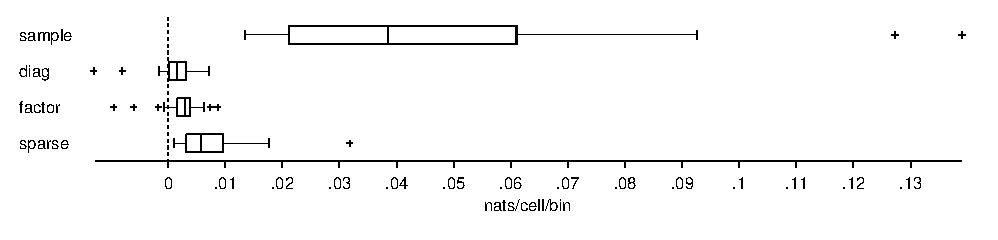
\includegraphics[width=\textwidth]{./figures/Figure3.eps}
        \end{center}
\caption[Evaluation of correlation estimators by cross-validation]
{{\bf Performance of estimator $C_{\sf sparse+latent}$ with respect to the normal loss function (eq.~\ref{eq:loss}) relative to the other estimators: $C_{\sf sample}$, $C_{\sf diag}$, $C_{\sf factor}$, and $C_{\sf sparse}$.}
Covariance estimators $C_{\sf sample}$, $C_{\sf diag}$, $C_{\sf factor}$, and $C_{\sf sparse}$ produced consistently greater validation losses than $C_{\sf sparse+latent}$ ($p<0.01$ in each comparison, Wilcoxon signed rank test, $n=27$ sites in 14 mice). The box plots indicate the $25^{th}$, $50^{th}$, and $75^{th}$ percentiles with the whiskers extending to the minimum and maximum values after excluding the outliers marked with `+'.
}\label{fig:3}
\end{fullpage}
\end{figure}
    %%%% FIGURE 3 from the paper

To test this hypothesis, we computed the relative cross-validation loss of estimators  $C_{\sf sample}$, $C_{\sf diag}$, $C_{\sf factor}$, and $C_{\sf sparse}$ with respect to $C_{\sf sparse+latent}$ in $n=27$ imaged sites in 14 mice.  The hyperparameters of each estimator were optimized by nested cross-validation (See Fig.~\ref{fig:S1} and  Methods). Indeed, the sparse+latent estimator outperformed the other estimators (Fig.~\ref{fig:3}). The respective median differences of the cross-validation loss were 0.039, 0.0016, 0.0029, and 0.0059 nats/cell/bin, significantly greater than zero ($p<0.01$ in each comparison, $n=27$ sites in 14 mice, Wilcoxon signed rank test).

\begin{figure}
\begin{fullpage}

        \begin{center}
        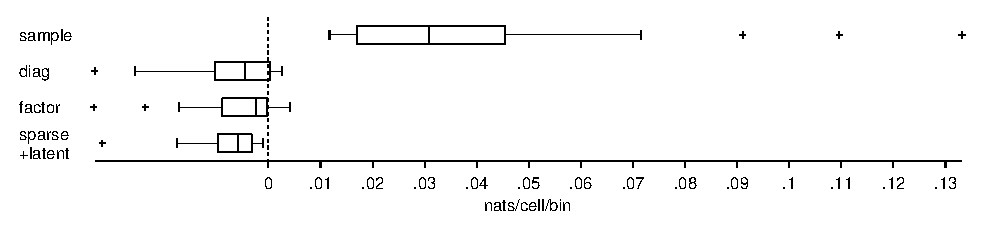
\includegraphics[width=\textwidth]{./figures/Supp02.eps}
        \end{center}

\caption[Performance evaluation of correlations estimators with respect to quadratic loss]{
{\bf Performance evaluation of correlation estimators with respect to quadratic loss.} 
The plot shows the quadratic loss (Eq.~\ref{eq:quad}) of estimator $C_{\sf sparse+latent}$ relative to the other estimators: $C_{\sf sample}$, $C_{\sf diag}$, $C_{\sf factor}$, and $C_{\sf sparse}$. All comparisons showed significant advantage of estimator $C_{\sf sparse+latent}$ ($p<10^{-3}$ in each comparison, Wilcoxon signed rank test, $n=27$ sites in 14 mice.
}\label{fig:S2}
\end{fullpage}
\end{figure}
  %%%%%% FIGURE 4 from the paper

The same evaluation based on the quadratic loss function,
\begin{equation}\label{eq:quad}
\loss{C,C_{\sf sample}^\prime}=\frac 1 {p^2}\Tr(C^{-1}C_{\sf sample}^\prime-I)^2,
\end{equation}
instead of the normal loss function reproduced the same relationship between the estimators (Fig.~\ref{fig:S2}). This suggests that the results of this study are robust to the choice of the loss function and do not depend on the assumption of gaussianity.

\subsection{Structure of $C_{\sf sparse+latent}$ estimates}

\begin{figure}
\begin{leftfullpage}
\caption[Example of partial correlation structure]{
{\bf Example of partial correlation structure from $C_{\sf sparse+latent}$.}
{\bf A, B.} The regularized estimate $C_{\sf sparse+latent}$ closely approximates the sample correlation matrix $C_{\sf sample}$.
{\bf C, D.} The partial correlation matrices from the two estimates differ substantially.
{\bf E.} The partial correlation matrix of the regularized estimate is decomposed into a sparse component with 92.8\% off-diagonal zeros (bottom-left) and low-rank component of rank 72 (top-right).
{\bf F.} The sparse component of the regularized partial correlation matrix had little resemblance to the sample correlations: The gray region indicates the range of correlations containing 92.8\% of cells pairs, equal to the fraction of zeros in the sparse partial correlation matrix. Correlation coefficients outside this interval formed the network of greatest correlations.  This network differed from the sparse component of the $C_{\sf sparse+latent}$:  Only 27.7\% of the highest correlations coefficients outside the gray regions coincided with interactions inferred by $C_{\sf sparse+latent}$.
{\bf G.} A graphical depiction of the positive (green) and negative (magenta) sparse partial correlations as edges between observed neurons. The line density is proportional to the magnitude of the partial correlation.
{\bf H.} A subset of neurons from the center of the cluster shown in {\bf G} showing the sparse partial correlations.
{\bf I.} The same subset of neurons with edges indicating sample correlations thresholded to match the sparsity of the sparse partial correlation. These edges correspond to the sample correlation coefficients outside the gray region in panel F.
}\label{fig:4}
\end{leftfullpage}
\end{figure}

\begin{figure}
\begin{fullpage}
        \begin{center}
        \includegraphics[height=\textwidth]{./figures/Reconstruction.pdf}
        \end{center}
\end{fullpage}
\end{figure}
  %%%%%% FIGURE 4 from the paper

\begin{figure}
\begin{fullpage}
    \begin{center}
        \includegraphics{./figures/Stats.pdf}
    \end{center}

\begin{caption}[Properties of functional connectivity across datasets]
{\bf Properties of functional connectivity across datasets.}
Each point represents an imaged site with its color indicating the population size as shown in panels A and B. The example site from Figures \ref{fig:2} and \ref{fig:4} is circled in blue.
\\
{\bf A.} The number of inferred latent units \emph{vs.}~population size.
{\bf B.} The connectivity of the sparse component of partial correlations as a function of population size.
{\bf C.} The average sample correlations \emph{vs.}~the average partial correlations (Eq.~\ref{eq:partial}) of the $C_{\sf sparse+latent}$ estimate.
{\bf D.} The percentage of negative interactions vs.~connectivity in the $C_{\sf sparse+latent}$ estimates.

\end{caption} \label{fig:5}

\end{fullpage}
\end{figure}
  %%%%%%% FIGURE 5 from the paper 

We examined the composition of the $C_{\sf sparse+latent}$ estimates at each imaged site (Fig.~\ref{fig:4} and Fig.~\ref{fig:5}). Although the regularized estimates were similar to the sample correlation matrix (Fig.~\ref{fig:4} A and B), the corresponding partial correlation matrices differed substantially (Fig.~\ref{fig:4} C and D). The estimates separated two sources of correlations: a network of linear interactions expressed by the sparse component of the inverse and latent units expressed by the low-rank components of the inverse (Fig.~\ref{fig:4} E). The sparse partial correlations revealed a network that differed substantially from the network composed of the greatest coefficients in the sample correlation matrix (Fig.~\ref{fig:4} F, G, H, and I).

In the example site (Fig.~\ref{fig:4}), the sparse component had 92.8\% sparsity (or conversely, 7.2\% connectivity: $\mbox{connectivity}=1-\mbox{sparsity}$) with average node degree of 20.9 (Fig.~\ref{fig:4} G). The average node degree, \emph{i.e.}\;the average number of interactions linking each neuron, is related to connectivity as $\mbox{degree} = \mbox{connectivity}\cdot(p-1)$, where $p$ is the number of neurons. The low-rank component had rank 72, denoting 72 inferred latent units. The number of latent units increased with population size (Fig.~\ref{fig:5} A) but the connectivity was highly variable (Fig.~\ref{fig:5} B): Several sites, despite their large population sizes, were driven by latent units and had few pairwise interactions. This variability may be explained by differences in brain states and recording quality and warrants further investigation.

The average partial correlations calculated from these estimates according to Eq.~\ref{eq:partial} at all 27 sites were about 5 times lower than the average sample correlations (Fig.~\ref{fig:5} C). This suggests that correlations between neurons build up from multiple chains of smaller interactions. Furthermore, the average partial correlations were less variable: the coefficient of variation of the average sample correlations across sites was 0.45 whereas that of the average partial correlations was 0.29, with larger populations exhibiting greater uniformity of average partial correlations than the smaller populations.

While the sample correlations were mostly positive, the sparse component of the partial correlations (`interactions') had a high fraction (28.7\% in the example site) of negative values (Fig.~\ref{fig:4} F). The fraction of negative interactions increased with the inferred connectivity (Fig.~\ref{fig:5} D), suggesting that negative interactions can be inferred only after a sufficient density of positive interactions has been uncovered.

Thresholded sample correlations have been used in several studies to infer pairwise interactions \citep{Golshani:2009, Feldt:2011, Malmersjo:2013, Sadovsky:2014}.  We therefore compared the interactions in the sparse component of $C_{\sf sparse+latent}$ to those obtained from the sample correlations thresholded to the same level of connectivity. The networks revealed by the two methods differed substantially. In the example site with 7.2\% connectivity in $C_{\sf sparse+latent}$, only 27.7\% of the connections coincided with the above-threshold sample correlations (Fig.~\ref{fig:4} F, H, and I). In particular, most of the inferred negative interactions corresponded to low sample correlations (Fig.~\ref{fig:4} F) where high correlations should be expected given the rest of the correlation matrix.

\subsection{Relationship of $C_{\sf sparse+latent}$ to orientation tuning and physical distances}

\begin{figure}
\begin{fullpage}
        \begin{center}
        \includegraphics[width=\textwidth]{./figures/OrientationAndDistance.pdf}
        \end{center}
\begin{caption}[Relationship between functional connectivity and circuit architecture]
{\bf Relationship between functional connectivity and circuit architecture.} 
The error bars mark the standard errors of the means. Five sites with highest connectivity (see Fig.~\ref{fig:5} B) were selected for this analysis.
{\bf A--C.} Normalized mean sample correlations (black) and normalized mean partial correlations (red) estimated by $C_{\sf sparse+latent}$ across $n=5$ imaged sites. The values in each bin are normalized by the means across the entire site, shown in Fig.~\ref{fig:5} C, to make the effects more comparable across the sites.
{\bf A.} Mean partial correlations in $C_{\sf sparse+latent}$ depend on $\Delta ori$ more strongly than mean sample correlations.
{\bf B.} Mean partial correlations in $C_{\sf sparse+latent}$ depend on $\Delta x$ more strongly than mean sample correlations. Only horizontally aligned cell pairs with $\Delta z<30\,\mu m$ were considered.
{\bf C.} Mean partial correlations in $C_{\sf sparse+latent}$ depend on $\Delta z$ more strongly than mean sample correlations. Only vertically aligned cell pairs with $\Delta x<30\,\mu m$ were considered.    {\bf D--F.} Normalized positive connectivity (green) and normalized negative connectivity (dark red) inferred by the $C_{\sf sparse+latent}$ estimator in $n=5$ imaged sites.
Here ``connectivity'' refers to the fraction of the non-zero elements in the sparse component $S$ of the $C_{\sf sparse+latent}$ estimator, which describes inferred direct interactions between specific pairs of the recorded neurons. Positive and negative connectivities refer to the fractions of the positive and negative partial correlations computed from  $S$, respectively.  ``Normalized positive connectivity'' is the ratio of the positive connectivity for pairs meeting a given condition, \emph{e.g.}~similar tuning with $\Delta ori <15^{\circ}$, to the average connectivity over the entire site.  Normalized negative connectivity is computed similarly for the negative connectivity.  The average connectivity across sites is shown in Fig.~\ref{fig:5} B with only the five most connected sites included in the analysis.  The normalization made the effects of tuning and distance more comparable across sites.
{\bf D.} Positive connectivity decreases with $\Delta ori$ whereas negative connectivity does not.
{\bf E.} Positive connectivity decays with $\Delta x$ whereas negative connectivity does not, within the examined range.
{\bf F.} Positive connectivity decays with $\Delta z$. Negative connectivity does not decay for small values of $\Delta z$.

\end{caption} \label{fig:6}

\end{fullpage}
\end{figure}
  %%%%%%%%% FIGURE 6 from the paper

We examined how the structure of the $C_{\sf sparse+latent}$ estimates related to the differences in orientation preference and to the physical distances separating pairs of cells (Fig.\;\ref{fig:6}).  Five sites with highest pairwise connectivities were included in the analysis. Partial correlations were computed using Eq.~\ref{eq:partial} based on the regularized estimate, including both the sparse and the latent component. Connectivity was computed as the fraction of pairs of cells connected by non-zero elements (interactions) in the sparse component of the estimate, distinguishing between the positive and negative connectivities.

First, we analyzed how correlations and connectivity depended on the difference in preferred orientations ($\Delta ori$) of pairs of significantly ($\alpha=0.05$) tuned cells. The partial correlations decayed more rapidly with $\Delta ori$ than did sample correlations ($p<10^{-9}$ in each of the five sites, two-sample $t$-test of the difference of the linear regression coefficients). Positive connectivity decreased with $\Delta ori$ ($p<0.005$ in each of the five sites, $t$-test on the logistic regression coefficient) whereas negative connectivity did not decrease (Fig.~\ref{fig:6} D): The slope in the logistic model of connectivity with respect to $\Delta ori$ was significantly higher for positive than for negative interactions ($p<0.04$ in each of the five sites, two-sample $t$-test of the difference of the logistic regression coefficient).

Second, we compared how correlations and connectivity depended on the physical distance separating pairs of cells. We distinguished between lateral distance, $\Delta x$, in the plane parallel to the pia, and vertical distance, $\Delta z$, orthogonal to the pia.  When considering the dependence on $\Delta x$, the analysis was limited to cell pairs located at the same depth with $\Delta z < 30\,\mu\mbox{m}$; conversely, when considering the dependence on $\Delta z$, only vertically aligned cell pairs with $\Delta x < 30\,\mu\mbox{m}$ were included. Again, the partial correlations decayed more rapidly both laterally and vertically than sample correlations ($p<10^{-6}$ in each of the five sites, for both lateral and vertical distances, two-sample $t$-test of the difference of the linear regression coefficients).
Positive connectivity decayed with distance ($p<10^{-6}$ in each of the five sites for positive interactions and $p<0.05$ for negative interactions, $t$-test on the logistic regression coefficient) (Fig.~\ref{fig:6} E), so that cells separated laterally by less than 25 $\mu\mbox{m}$ were 3.2 times more likely to be connected than cells separated laterally by more than 150 $\mu\mbox{m}$. Although the positive connectivity appeared to decay faster with vertical than with lateral distance, the differences in slopes of the respective logistic regression models were not significant with available data. The negative connectivity decayed slower with distance (Fig.~\ref{fig:6} E and F): The slope in the respective logistic models with respect to the lateral distance was significantly higher for positive than for negative connectivities ($p<0.05$ in each of the five sites, two-sample $t$-test of the difference of the logistic regression coefficients).

\section*{Discussion}
\subsection*{Functional connectivity as a network of pairwise interactions}
Functional connectivity is often represented as a graph of pairwise interactions. The goal of many studies of functional connectivity has been to estimate  anatomical connectivity from  observed multineuronal spiking activity.  For example, characteristic peaks and troughs in the pairwise cross-correlograms of recorded spike trains contain statistical signatures of directional monosynaptic connections and shared synaptic inputs \citep{Gerstein:1964, Perkel:1967, Moore:1970, Alonso:1998, Denman:2013}.  Such signatures are ambiguous as they can arise from network effects other than direct synaptic connections \citep{Aertsen:1989}.  With simultaneous recordings from more neurons, ambiguities can be resolved by inferring the conditional dependencies between pairs of neurons.  Direct causal interactions between neurons produce statistical dependency between them even after conditioning on the state of the remainder of the network and external input. Therefore, conditional independence can signify the absence of a direct causal influence.

Conditional dependencies can be inferred by fitting a probabilistic model of the joint population activity. For example, generalized linear models (GLMs) have been constructed to  include biophysically plausible synaptic integration, membrane kinetics, and individual neurons' stimulus drive~\citep{Pillow:2008}.  Maximum entropy models constrained by observed pairwise correlations are among other models with pairwise coupling between cells \citep{Schneidman:2006, Tkacik:2006, Yu:2008, Tang:2008, Shlens:2009}.  Assuming that the population response follows a multivariate normal distribution, the conditional dependencies between pairs of neurons are expressed by the partial correlations between them.   Each probabilistic model, fitted to the same data may reveal a completely different network of `interactions',  \emph{i.e.}\;conditional dependencies between pairs of cells.

It is not yet clear which approach provides the best correspondence with anatomical connectivity. Little experimental evidence is available to answer this question.  The connectivity graphs inferred by various statistical methods are commonly reported without examining their relation to anatomy.
Topological properties of such graphs have been interpreted as principles of circuit organization (\emph{e.g.} small-world organization) \citep{Feldt:2011, Yu:2008, Malmersjo:2013, Sadovsky:2014}.  However, the topological properties of functional connectivity graphs can depend on the method of inference \citep{Zalesky:2012}. Until a physiological interpretation of functional connectivity is established, the physiological relevance of such analyses remains in question and we did not attempt them here.

Inference of the conditional dependencies also depends on the completeness of the recorded population:  To equate conditional dependencies to direct interaction between neurons, we must record from all neurons with which the pair interacts. Unobserved portions of the circuit may manifest as conditional dependencies between observed neurons that do not interact. For this reason, statistical models of population activity have been most successfully applied to \emph{in vitro} preparations of the retina or cell cultures where high-quality recordings from the complete populations were available \citep{Pillow:2008}. In cortical tissue, electrode arrays record from a small fraction of cells in a given volume, limiting the validity of inference of the pairwise conditional dependencies. Perhaps for this reason, partial correlations have not, until now, been used to describe the functional connectivity in cortical populations.

Two-photon imaging of population calcium signals presents unique advantages for the estimation of functional connectivity.  While the temporal resolution of calcium signals is limited by calcium dye kinetics, fast imaging techniques combined with spike inference algorithms provide millisecond-scale temporal resolution of single action potentials \citep{Grewe:2010}. However, such high temporal precision comes at the cost of the accuracy of inferred spike rates.  Better accuracy is achieved when calcium signals are analyzed on scales of tens of milliseconds \citep{Cotton:2013}.  The major advantage of calcium imaging is its ability to characterize the spatial arrangement and types of recorded cells.  Recently, advanced imaging techniques have allowed recording from nearly every cell in a volume of cortical tissue  \emph{in vivo} \citep{Katona:2012, Cotton:2013} and even from entire nervous systems \citep{Leung:2013, Ahrens:2013}.  These techniques may provide more incisive measurements of functional connectivity than electrophysiological recordings.

The low temporal resolution of calcium signals limits the use of functional connectivity methods that rely on millisecond-scale binning of signals (cross-correlograms, some GLMs, and binary maximum entropy models).  Hence, most studies of functional connectivity have relied on instantaneous sample correlations \citep{Greenberg:2008, Golshani:2009, Hofer:2011, Malmersjo:2013} .  Although some investigators have interpreted such correlations as indicators of (chemical or electrical) synaptic connectivity, most used them as more general indicators of functional connectivity without relating them to underlying mechanisms.

In this study, we sought to infer pairwise functional connectivity networks  in cortical microcircuits. We hypothesized that partial correlations correspond more closely to underlying mechanisms than sample correlations when recordings are sufficiently dense.  Since neurons form synaptic connections mostly locally and sparsely \citep{Perin:2011}, we \emph{a priori} favored solutions with sparse partial correlations.  Under the assumptions that the recorded population is sufficiently complete and that the model correctly represents the nature of interactions, the network of partial correlations can be hypothesized to be a better representation of functional dependencies than correlations.

\subsection*{Functional connectivity as coactivations}
Another approach to describing the functional connectivity of a circuit is to isolate individual patterns of multineuronal coactivations \citep{Gerstein:1989, Chapin:1999, Peyrache:2010, Ch:2010, Lopes:2011, Lopes:2013}. Depending on the method of their extraction, coactivation patterns may be referred to as \emph{assemblies}, \emph{factor loadings}, \emph{principal components}, \emph{independent components}, \emph{activity modes}, \emph{eigenvectors}, or \emph{coactivation maps}. Coactivation patterns could be interpreted as signatures of Hebbian cell assemblies \citep{Gerstein:1989, Ch:2010}, \emph{i.e.}\;groups of tightly interconnected groups of cells involved in a common computation.  Coactivation patterns could also result from shared input from unobserved parts of the circuit, or global network fluctuations modulating the activity of the local circuit \citep{Okun:2012}.

Coactivation patterns and pairwise connectivity are not mutually exclusive since assemblies arise from patterns of synaptic connectivity.  However, an analysis of coactivation shifts the focus from detailed interactions to  collective behavior.
In our study, the functional connectivity solely through modes of coactivations was represented by the factor analysis-based estimator $C_{\sf factor}$.

\subsection*{Combining pairwise interactions and coactivations}
In the effort to account for the joint activity patterns that are poorly explained by pairwise interactions, investigators have augmented models of pairwise interactions with additional mechanisms such as latent variables \citep{Koster:2013},  high-order correlations \citep{Ganmor:2011}, or global network fluctuations \citep{Tkacik:2013}.

In our study, we combined pairwise interactions with collective coactivations by applying the recently developed numerical techniques for the inference of the partial correlation structure in systems with latent variables \citep{Chandrasekaran:2010, Ma:2013}.  The resulting estimator, $C_{\sf sparse+latent}$, effectively decomposed the functional connectivity into a sparse network of pairwise interactions and coactivation mode vectors.

\subsection*{Addressing ill-posedness}
Inferring the conditional dependencies between variables in a probabilistic model is an ill-posed problem: small variations in the data produce large errors in the inferred network of dependencies. The problem becomes worse as the number of  recorded neurons increases until such models lose their statistical validity \citep{Roudi:2009}.  As techniques have improved to allow recording from larger neuronal populations, experimental neuroscientists have addressed this problem by extending the recording durations to keep sampling noise in check and verified that existing models are not overfitted \citep{Tkacik:2013}. However, ambitious projects, such as the BRAIN initiative  \citep{Alivisatos:2013}, aim to record from significantly larger populations. Simply increasing recording duration will not be sufficient, and the problem must be addressed by using regularized estimators. Regularization biases the solution toward a small subspace in order to counteract the effect of  sampling noise in the empirical data. However, biasing the solution to an inappropriate subspace does not allow significant estimation improvement and hinders interpretation.

Several strategies have been developed to limit the model space in order to improve the quality of the estimate. For example, Ganmor et al. \citep{Ganmor:2011} developed a heuristic rule to identify the most significant features that must be fitted by a maximum entropy model for improved performance in the retina. As another example of regularization, generalized linear models typically employ $L_1$ penalty terms to constrain the solution space and to effectively reduce the dimensionality of the solution \citep{Pillow:2008}.

In our study, regularizations were accomplished by dimensionality reduction (feature selection) schemes to produce sparse, constrained solutions. Only the most efficient scheme was considered in the analysis of functional connectivity.

\subsection*{Model selection}
Various model selection criteria have been devised to select between families of models and the optimal subsets of variables in a given model family based on observed data. Despite its computational requirements, cross-validation is among the most popular model selection methods due to its minimal assumptions about the data generating process \citep{Arlot:2010}.

We evaluated the covariance matrix estimators a loss function based on multivariate normal log likelihood.  However, this does not limit the applicability of its conclusions to normal distributions. Indeed our major findings could be reproduced using other loss functions (compare Fig.~\ref{fig:3} and Fig.~S2).  Other probabilistic models, fitted to the same data, could also serve as estimators of the covariance matrix.  If a different model yields better estimation of the covariance matrix than the estimator proposed here, we believe that its structure should deserve consideration as the better representation of the functional connectivity.

The results of model selection must be interpreted with caution.  As we demonstrated by simulation, even models with incorrect forms of dependencies can substantially improve estimates (Fig.~\ref{fig:1}). Therefore, showing that a more constrained model has better cross-validated performance than a more complex model does not necessarily support the conclusion that it reveals a better representation of dependencies in the data.  This caveat is related to \emph{Stein's Paradox} \citep{Efron:1977}: The biasing of an estimate toward an arbitrary low-dimensional target can consistently outperform a less constrained estimate.

\subsection*{Physiological interpretation and future directions}

We showed that among several models a sparse network of linear interactions with several latent inputs yielded the best estimates of the noise covariance matrix for cortical microcircuits.  This finding is valuable in itself: improved estimates of the noise covariance matrix for large datasets are important in order to understand the role of noise correlations in population coding \citep{Abbott:1999, Sompolinsky:2001, Averbeck:2006, Ecker:2011}

Moreover, this estimation approach provides a graphical representation of the dependencies in the data that can be used to formulate and test hypotheses about the structure of connectivity in the microcircuit. Importantly, the inferred functional interactions were substantially different from the network of the highest sample correlations.  For example, the $C_{\sf sparse+latent}$ estimator reveals a large number of negative interactions that were not present in the sample correlation matrix (Fig.~\ref{fig:4} F) and may reflect inhibitory circuitry.

Distances between cells in physical space and in sensory feature space had a stronger effect on the partial correlations estimated by the $C_{\sf sparse+latent}$ estimator than on sample correlations (Fig.~\ref{fig:6} A--C).
These differences support the idea that correlations are built up from partial correlations in chains of intermediate cells positioned closer and tuned more similarly to one another, with potentially closer correspondence to anatomical connectivity.  These differences may also be at least partially explained by a trivial effect of regularization: the $L_1$ penalty applied by the estimator (Eq.~\ref{eq:ma}) suppresses small partial correlations to greater extent than large partial correlations, enhancing the apparent effect of distance and tuning.  Distances between cells in physical space and in sensory feature space also had distinct effects on the positive and negative connectivities inferred by the estimator (Fig.~\ref{fig:6} D--F); we could not think of a numerical artifact that could produce this effect. The distinct positive and negative connectivity patterns  may reflect geometric and graphical features of local excitatory and inhibitory networks. Indeed, the relationships between patterns of positive and negative connectivities inferred by the estimator mirrored the properties of excitatory and inhibitory synaptic connectivities with respect to distance, cortical layers, and feature tuning \citep{Song:2005, Oswald:2008, Adesnik:2010, Perin:2011, Fino:2011, Hofer:2011, Isaacson:2011, Levy:2012}. For example, while excitatory neurons form synapses within highly specific local cliques \citep{Perin:2011}, inhibitory interneurons form synapses with nearly all excitatory cells within local microcircuits \citep{Fino:2011, Hofer:2011, Packer:2011}.  To further investigate the link between synaptic connectivity and inferred functional connectivity, in future experiments, we will use molecular markers for various cell types with follow-up multiple whole-cell \emph{in vitro} recordings \citep{Hofer:2011, Ko:2013} to directly compare the inferred functional connectivity graphs to the underlying anatomical circuitry. Finally, the latent units inferred by the estimator can be analyzed for their physiological functions. For example, these latent units may be modulated under different brain states (e.g. slow-wave sleep, attention) and stimulus conditions (e.g. certain types of stimuli may engage feedback connections).

\section{Materials and Methods}

\subsection{Ethics statement}
All procedures were conducted in accordance with the ethical guidelines of the National Institutes of Health and were approved by the Baylor College of Medicine IACUC.

\subsection{Surgery and two-photon imaging}
The surgical procedures and data acquisition were performed as described in \citep{Cotton:2013}: C57BL/6J mice (aged p40--60) were used. Anesthesia was initiated with isoflurane (3\%) and maintained with the mixture of fentanyl (0.05 mg/kg), midazolam (5 mg/kg), and medetomidine (0.5 mg/kg), with boosts of half the initial dose every 3 hours.  A craniotomy was performed over the right primary visual cortex.  Membrane-permeant calcium indicator Oregon Green 488 BAPTA-1 AM (OGB-1, Invitrogen) was loaded by bolus injection.  The craniotomy was sealed using a glass coverslip secured with dental cement.

Calcium imaging began 1 hour after dye injection.  All imaging was performed using 3D-RAMP two-photon microscopy \citep{Cotton:2013}. First, a 3D stack was acquired and cells were manually segmented. Then calcium signal were collected by sampling in the center of each cell at rates of 100 Hz or higher, depending on the number of cells.

\subsection{Visual stimulus}
The visual stimulus consisted of full-field drifting gratings with 90\% contrast, luminance of 10 cd/m$^2$, spatial frequency of 0.08 cycles/degree, and temporal frequency of 2 cycles/s. Two types of stimuli were presented for each imaging site: First, directional tuning was mapped using a pseudo-random sequence of drifting gratings at sixteen directions of motion, 500 ms per direction, without blanks, with 12--30 trials for each direction of motion.  Second, ro measure correlations, the stimulus was modified to include only two directions of motion (in 9 datasets) or five directions (in 22 datasets) and the gratings were presented for 1 second and were separated by 1-second blanks, with 100--300 trials for each direction of motion.

\subsection{Data processing}
All data were processed in MATLAB using the DataJoint data processing chain toolbox (http://datajoint.github.com).

The measured fluorescent traces were deconvolved to reconstruct the firing rates for each neuron: First, the first principal component was subtracted from the raw traces in order to reduce common mode noise related to small cardiovascular movements \citep{Cotton:2013}. The resulting traces were high-pass filtered above 0.1 Hz and downsampled to 20 Hz (Fig.~\ref{fig:2} C). Then, the firing rates were estimated using by nonnegative deconvolution \citep{Vogelstein:2010}.

Orientation tuning was computed by fitting the mean firing rates for each direction of motion $\phi$ using two-peaked von Mises tuning functions $f(\phi)=a + b\exp\left[\frac 1 w(\cos(\phi-\theta)-1) \right] + c\exp\left[\frac 1 w(\cos(\phi-\theta+\pi)-1) \right]$ where $b\ge c$ are the amplitudes of the two respective peaks, $w$ is the tuning width, and  $\theta$ is the preferred direction. The significance of the fit was determined by the permutation test: the labels of the direction were randomly permuted 10,000 times; the $p$-values of the fits were computed as the fraction of permutations that yielded $R^2$ equal to or higher than that of the original data.  Cells were considered tuned with $p<0.05$.

For covariance estimation, the analysis was limited to the period with 2 or 5 stimulus conditions and lasted between 14 and 27 minutes (mean 22 minutes).  Cells that did not have substantial spiking activity (those whose variance was less than 1\% of the median across the site) or whose activity was unstable (those whose variance in the least active quarter of the recording did not exceed 1\% of the variance in the most active quarter) were excluded from the analysis.

\subsection{Cross-validation}
To compare the performance of the estimators, we used conventional 10-fold cross-validation: Trials were randomly divided into 10 subsets with approximately equal numbers of trials of each condition in each subset. Each subset was then used as the testing sample with the rest of the data used as the training sample for estimating the covariance matrix. The average validation loss over the 10 folds was reported.

Since each of the regularized estimators had one or two hyperparameters, we used \emph{nested cross-validation}:  The outer loop evaluated the performance of the estimators with the hyperparameter values optimized by cross-validation within the inner loop.  Hyperparameters were optimized by a two-phase search algorithm: random search to find a good starting point for the subsequent pattern search to find the global minimum.  The inner cross-validation loop subdivided the training dataset from the outer loop to perform 10-fold cross-validation in order to evaluate each choice of the hyperparameter values.  Thus the size of the training dataset within the inner loop comprised 81\% of the entire recording. Fig.~S1 illustrates the dependence of the validation loss on the hyperparameters of the $C_{\sf sparse+latent}$ estimator for the example site shown in Figures \ref{fig:2} and \ref{fig:4} and the optimal value found by the pattern search algorithm.

When the validation loss was not required, only the inner loop of cross-validation was used on the entire dataset.  This approach was used to compute the covariance matrix estimates and their excess loss in the simulation study (Fig.~\ref{fig:1} Rows 4 and 5) and to analyze the partial correlation structure of the $C_{\sf sparse+latent}$ estimator (Fig.~\ref{fig:4}--\ref{fig:6}).

\subsection{Covariance estimation}
Within the inner loop of cross-validation, regularized covariance matrix estimation required only the sample covariance matrix $C_{\sf sample}$ of the training dataset and the hyperparameter values provided by the outer loop.

Estimator $C_{\sf diag}$ (Eq.~\ref{eq:c-diag})  used two hyperparameters: the covariance shrinkage intensity $\lambda \in [0,1]$ and variance shrinkage intensity $\alpha \in [0,1]$.  The variances (the diagonal of $C_{\sf sample}$) were shrunk linearly toward their mean value $\frac 1 p \Tr(C_{\sf sample})$:
\begin{equation}
D = (1-\alpha)C_{\sf sample}\circ I + \alpha \frac 1 p \Tr(C_{\sf sample}) I
\end{equation}
The $C_{\sf diag}$ estimate was then obtained by shrinking $C_{\sf sample}$ toward $D$ according to Eq.~\ref{eq:c-diag}.

In estimator $C_{\sf factor}$ (Eq.~\ref{eq:c-factor}), the low-rank matrix $L$ and the diagonal matrix $D$ are found by solving the minimization problem
\begin{equation}
(L,D) = \argmin\limits_{\hat L,\hat D} \loss{\hat L + \hat D,C_{\sf sample}},
\end{equation}
by an expectation-maximization (EM) algorithm with specified rank of $L$. Additional the diagonal matrix of individual variances is shrunk toward its mean value according to Eq.~\ref{eq:c-factor}.

In estimator $C_{\sf sparse}$ (Eq.~\ref{eq:c-sparse}), the sparse precision matrix $S$ is found by minimizing the $L_1$-penalized loss with regularization parameter $\lambda$:
\begin{equation}
S = \argmin\limits_{\hat S \succ 0} \loss{{\hat S}^{-1},C_{\sf sample}} + \lambda \|\hat S \|_1
\end{equation}
where $\hat S\succ 0$ denotes the constraint that $\hat S$ be a positive-definite matrix and $\|\hat S\|_1$ is the element-wise $L_1$ norm of the matrix $\hat S$. This problem formulation is known as \emph{graphical lasso} \cite{pMeinshausen:2006, Friedman:2008}. To solve this minimization problem, we adapted the alternative-direction method of multipliers (ADMM) \citep{Ma:2013}.
Unlike $C_{\sf diag}$ and $C_{\sf factor}$, this estimator does not include linear shrinkage: the selection of the sparsity level provides sufficient flexibility to fine-tune the regularization level.

Estimator $C_{\sf sparse+latent}$ (Eq.~\ref{eq:c-sl}) estimates a larger sparse precision matrix $S^\ast$ of the joint distribution of the $p$ observed neurons and $d$ latent units.
\begin{equation}
S^\ast=
\begin{pmatrix}
S & S_{12} \\
S_{12}^\T & S_{22}
\end{pmatrix},
\end{equation}
where the $p\times p$ partition $S$ corresponds to the visible units.
Then the covariance matrix of the observed population is
\begin{equation}
C_{\sf sparse+latent} = \left(S-S_{12}S_{22}^{-1}S_{12}^\T\right)^{-1}
\end{equation}
The rank of the $p\times p$  matrix $L=S_{12}S_{22}^{-1}S_{12}^\T$ matches the number of the latent units in the joint distribution. Rather than finding $S_{12}$ and $S_{22}$ separately, $L$ can be estimated as a low-rank matrix. We adapted the ADMM algorithm to minimize the loss function with $L_1$ penalty on $S$ to regulate its sparseness and nuclear norm penalty on $L$ to regulate its rank \citep{Chandrasekaran:2010,Ma:2013}:
\begin{equation}\label{eq:ma}
(S,L) = \argmin\limits_{\hat S,\hat L} \loss{\hat S-\hat L, C_{\sf sample}} + \alpha\|\hat S\|_1 + \beta\Tr(\hat L)
\end{equation}

The partial correlation matrix (Eq.~\ref{eq:partial}) computed from $C_{\sf sparse+latent}$ includes interactions between the visible and latent units and was used in Fig.~\ref{fig:4} C and D and Fig.~\ref{fig:5} C, and Fig.~\ref{fig:6} A--C).  The partial correlation matrix computed from $S$ alone expresses strengths of pairwise interactions
\begin{equation}
P_{\sf sparse} = -(S\circ I)^{-\frac 1 2} S  (S\circ I)^{-\frac 1 2}
\end{equation}
and were used in Fig.~\ref{fig:4} F, G, H.

The MATLAB code for these computations is available online at http://github.com/atlab/cov-est.
\subsection{Cross-validation with conditioned variances}
This study required an unbiased estimate of the discrepancy between various correlation matrix estimates and the true value of the correlation matrix. This was accomplished by cross-validation whereby regularized covariance matrix estimates computed from training samples were compared to unbiased covariance matrix estimates computed from independent testing samples. Loss functions were defined with respect to the covariance matrix rather than the correlation matrix because no unbiased estimate of the correlation matrix exists for finite sample sizes in the general case \citep{Fisher:1921}. In particular, we showed that with the normal loss function (Eq.~\ref{eq:loss}), the validation loss $\loss{C,C_{\sf sample}^\prime}$ is an unbiased estimate of true loss when $C_{\sf sample}^\prime$ is an unbiased estimate. However, this approach only worked under the assumption of uniform variances across all conditions included in the training and testing samples.  Here, we extend the validation loss to the estimation and evaluation of a common correlation matrix across multiple conditions with different variances.

Let $T_c$ and $T_c^\prime$ denote the time bin indices for the training and testing samples, respectively, limited to condition $c$. Here, the prime symbol marks quantities estimated from the testing sample.




\chapter{Differential functional connectivity of parvalbumin-positive cells}
\clearpage

\section{Introduction}
\citep{Hofer:2011, Packer:2011}
\section{Experimental Procedures}
\input{pv-labeling.tex}

\appendix

\chapter{Cross-validation with condition specific variances}
\bibliographystyle{dy-thesis-style}
\bibliography{biblio.bib}
\addcontentsline{toc}{chapter}{\numberline{}Bibliography}

\end{document}
